\chapter{Background in scientific literature}
\label{chapter:background} 

Here is a look to the releavant papers and such - I'll update this section once
I get to work with bibtex.

This section focuses on scientific literature.

\section{Open access publishing}
\label{sec:benefits_open_publishing}

Open access refers to the online literature, research data and research papers in the
context of this thesis, that are free of charge and openly available for reuse
and redistribution \cite{suber2007open}\cite{bailey2008open}. Research papers
have lived in the open access space for a much longer time and the research
shows that publishing research papers openly correlates to increased citations
(ranging between 36\% - 172\% increase \cite{DBLP:journals/corr/abs-cs-0606079},
\cite{harnad2004comparing}\cite{eysenbach2006citation}). Open access publishing of research papers make the
paper known and cited faster than non open access \cite{harnad2004comparing}.
The increase in citations to research papers is magnified in papers woth lower
ranked journals, implying that open access publishing is a cost effective way
to increase the chance of making research impact
\cite{DBLP:journals/oir/XiaN12}.

There are different ways to do open access to research papers. One division is
the Golden Road and the Green Road, where the former refers to the journals
themselves publishing with open access and the latter to so called
self-archiving, where researchers publish their papers themselves \cite{harnad2004access}.
Self-archiving can be done on the research paper's author personal website,
a disciplinary archive or a institutional repository (either an institution
wide or smaller unit, a department for example) \cite{bailey2008open}. Aalto
University has an institutional repository for research papers and theses
produced in Aalto University. It's available at \url{https://aaltodoc.aalto.fi/}.

Open access publishing is growing in popularity. A study that explored the
growth of open access publishing between years 1993-2009 reported an annual
growth rate of 18\% in open access journals and 30\% increase in open access
articles, shown in figure \ref{fig:oa_increase} \cite{laakso2011development}.
The study does not speculate on the reasons behind the growth of open access
publishing, but mentions the fact that nowadays many researchers use free
search engines such as Google Scholar (\url{https://scholar.google.fi/}) to
look for sources and that makes articles published openly to stand on equal
footing with other articles and they are more readily available. Open access
has also introduced the concept of open access mandate, which is a mandata or
a policy adopted by a university, research institution or researach funder.
The open access mandate means that the researchers working under the mandate
are rqeuired to publish their reserach papers. A list of such entities is
maintained at \url{http://roarmap.eprints.org/}. The mandate likely has
contributed to the increase in open access.

\begin{figure}
    \begin{centering}
        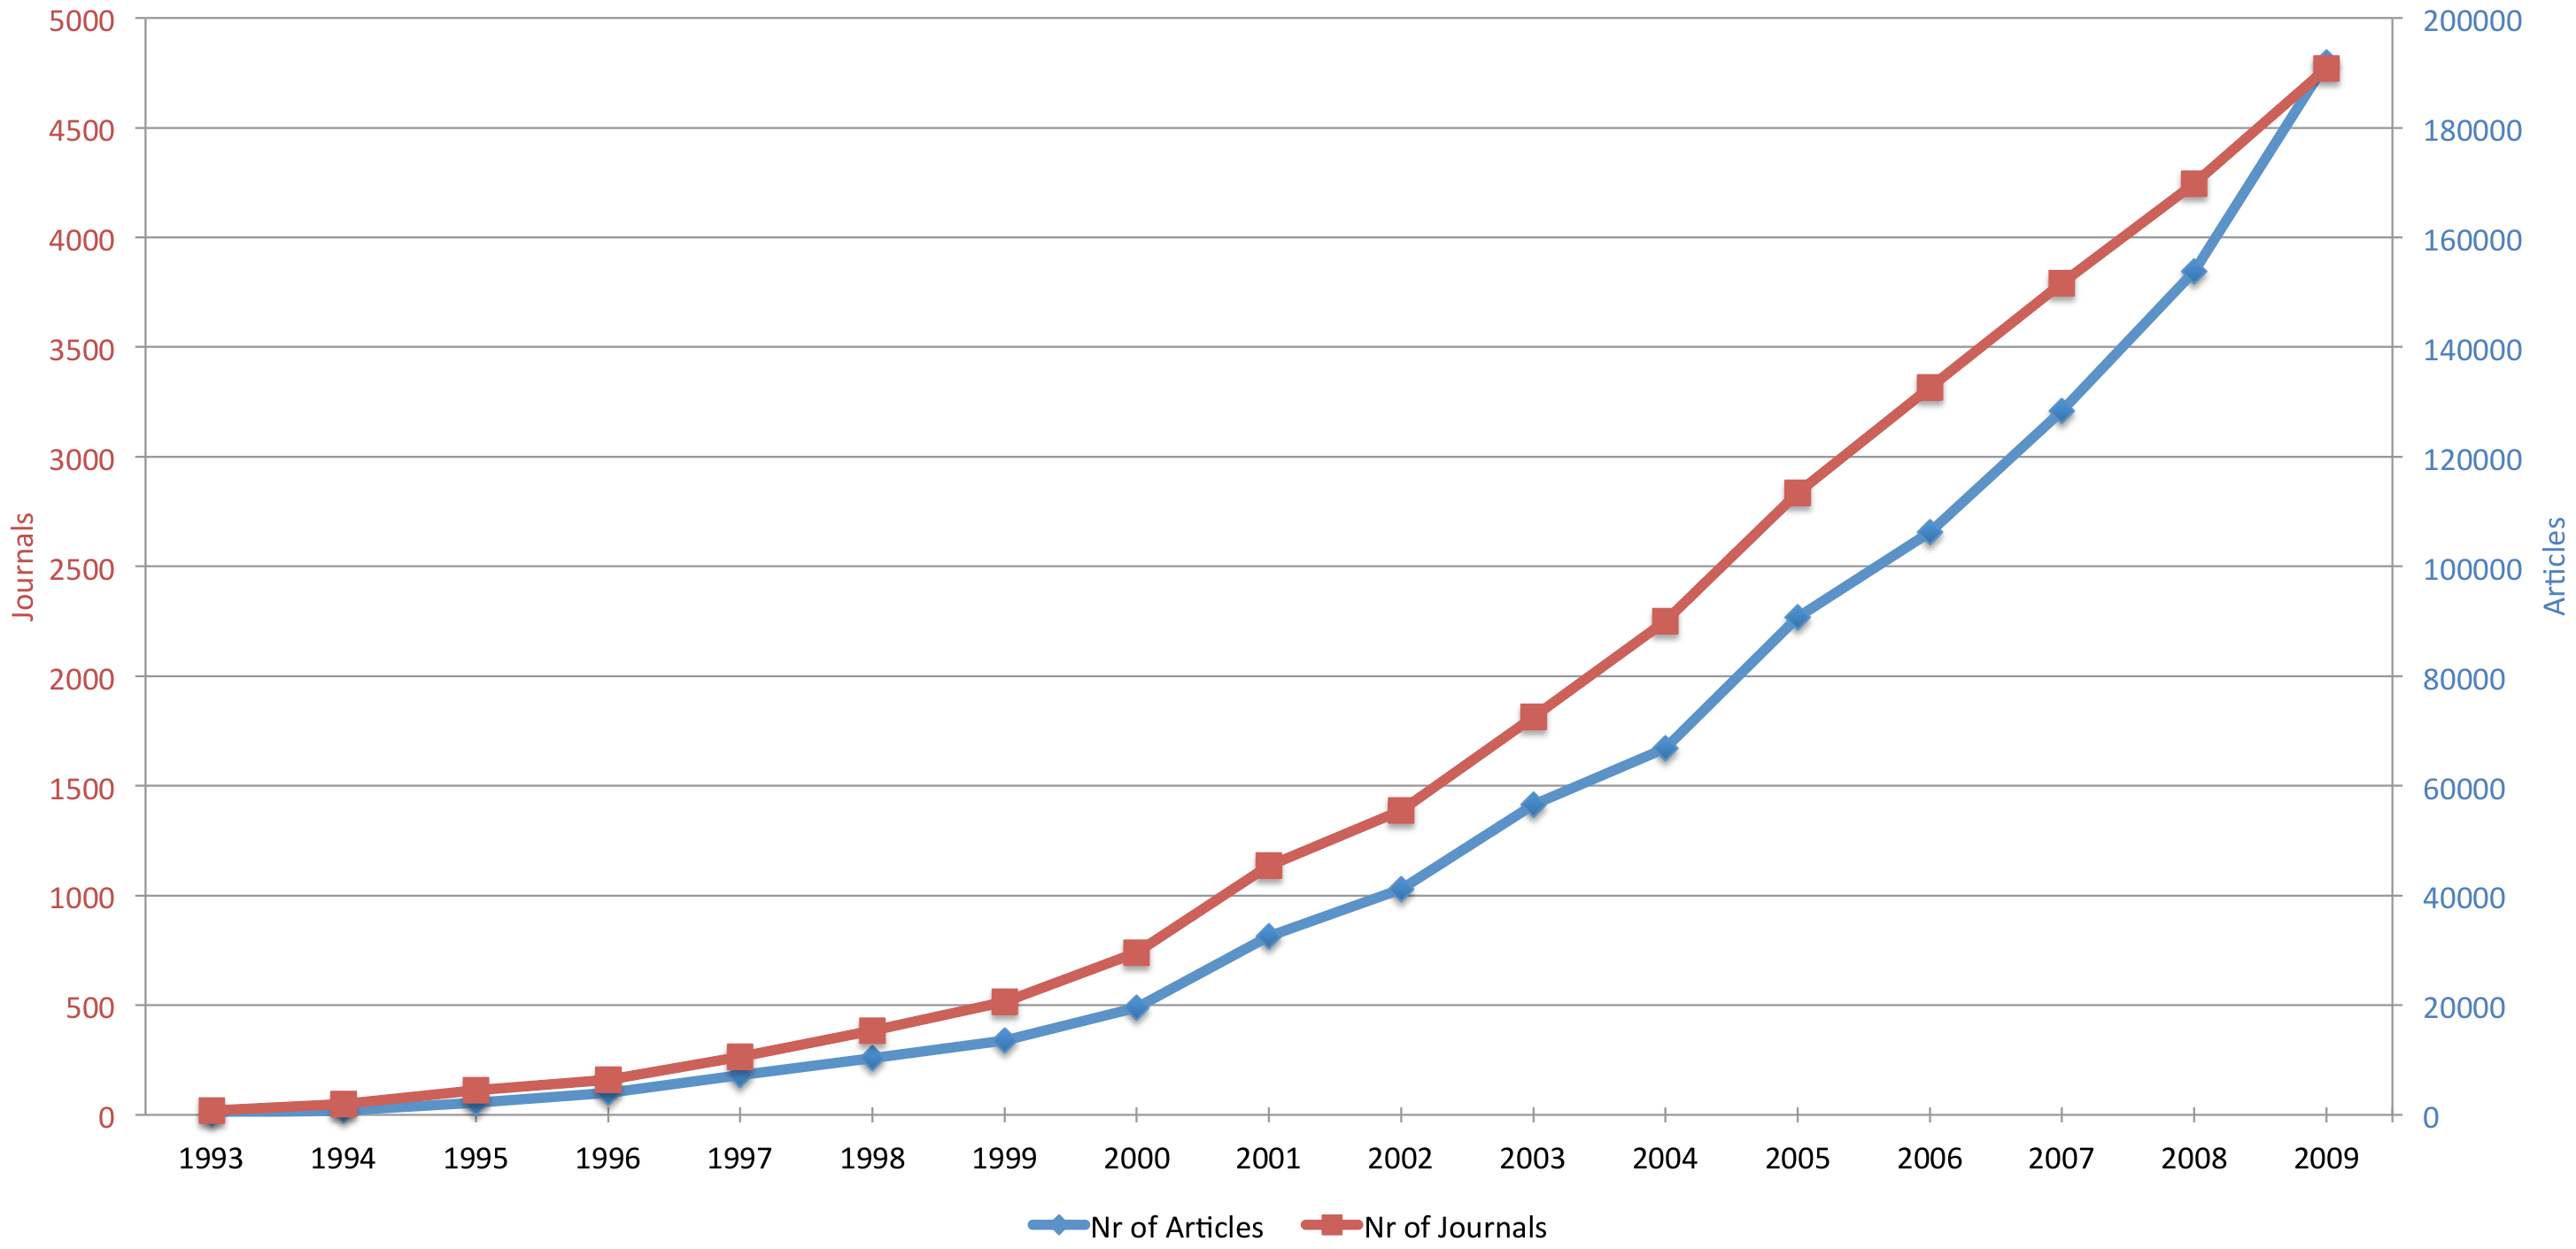
\includegraphics[width=\textwidth]{images/oa_increase}
    \end{centering}
    \caption{The growth of open access publishing between from 1993 to 2009 \cite{laakso2011development}}
    \label{fig:oa_increase}
\end{figure}

Open access publishing has been studied a lot, ranging from different
implementations (citation) to the effects of the Internet being a catalyst
for making open publishing posisble in a cost efficient large scale manner
(citation). Many nstitutions, such as universities, governments and other
funding bodies are advocating open access publishing (citation). Open access
is generally thought to increase the citation rate of a paper, making research
more impactful and since many studies are publicly funded, the perception is
that the results should be publicly funded as well.

This thesis focuses on publishing research data.

\section{The challenges of research data to open access}
\label{sec:research_data_oa}

Unlike reserch papers, research data is lacking in good guidelines and
practices to publish data in an open access way (citation). There is a
multitude of reasons behind that. The next sections (forward reference) will
describe those.

\subsection{Research data is diverse}

While research papers generally follow a
strict structure and can easily be published in a PDF format, research data
comes in all forms and flavors. For example, research data from a brain imaging
study will look completely different from a dataset that originates from
sociological research (citation). Not only the shape of the data is different,
the size of datasets can vary from the few megabyte survey results to the
multiple petabyte simulation results from a particle collider.

Even when you get down to practicalities the diversity of research data offers
challenges - results generated from one software might be binary incompatible
with another software within one field of science. And even if you were using
the same software, our versions might be different or you might do things in
such a different way that you are not compatible with other working on the
same field.

\subsection{Research data requires metadata}

Metadata refers to data about data. It's a rescription of the data and entails
details such as when was the dataset collected, what kind of equipement was
used or if there was something noteworthy in how the experiment was run
(citation). Due to the diversity of data in different fields, the metadata
differs between fields as well (citation). Some standards for metadata exist,
but not an all fields of science (citaiton).

Research data in and on itself is the most important thing to be published, but
working on someone else's research data without the relevant metadata adds
another layer of complexity and might mean that you cannot use the data at all
(citation). One reason to publish your data is to make reproduciton of you work
(citation) easier, and without proper metadata it is hard or impossible to
do that.

\subsection{Research data might be a privacy issue}

In many fields of science (healthcare, telecommunication to name a few) the
privacy of the participants to the studies is essential. If you go about
publishing your data, you need to be concious about maintaning the anonymity
of the people taking part in your research (citation).

\subsection{Research data might be published locally}

Due to privacty issues or maybe funding issues it might be so that the data
that is used in research cannot be published to the world but maybe you can
publish it within your orgnanization or upon request. This sets access rights
requirements to your dataset, so while you might be able to openly publish
your metadata in order to tell the world that your dataset exists, your dataset
should not be available for everyone (citation). 

\subsection{Research data requires support from higher ups and related partners}

Individuals can publish their data any way they wish as long as it's within
legal boundaries. However, if institutions such as universities or librareis
wish to venture into publishing their research, individual researchers and
people working with the data need support from their organizations. Studies
have shown (citation) that organizations need to commit to the idea of open
access publishing in order for it to work.

\section{Benefits of publishing research data}

The benefits of research data publishing are not as straightforward as
publishing papers. Academic credit is distributed by the number of papers you
publish and by the number of citations you get to those papers. Research data
is often viewed as the fuel to the research. The actual downsides, from the
reserach, are covered in the next section (forward reference).

\subsection{Publishing reserach data yields more citations}

One of the most direct upsides of publishing reserach data is that it seems to
increase the citation count of the paper where the published data was related
to (citation). The research on this has not been done on all fields of science,
but the numbers from the fields it hase been conducted (medical science and
some others, put them down here at a later date) are impressive - up to
69\% (citation) increase in citation rates.

\subsection{Publishing research data makes your reserach reach more people}

While being quite intuitive, it's worth mentioning that open publishing of
research data results in your research being exposed to a larger audience
(citation).

\subsection{Publishing reserch data grows the impact of your research}

The impact of one's research is hard to quantify, but exposing more people to
your research and at the same time promoting your research papers enables your
research find places where it can make difference in the world (citation).
(this small section requires more meat on the bones)

\subsection{Publishing research data makes your research better quality}

The scientific principles require all scientific work to be replicateable. It
is quite hard to replicate your results just based on your paper, especially if
your paper is heavy on analysis dependant on your data (citations). In this
light publishing your research data in fact makes your research better quality.

Publishing research data should make all research data better as well. The
logic behind this is that if all research data was public, it would fall under
public scrutiny making it harder to publish fraudulent results and it would
force the authors of the data to make it more readable to the wider audience
(citation).

\subsection{Publishing research data can save you from fraud accusitions}

In addition to preventing fraud from others, if your data is public you could
easily deal with fraud accusitions by pointing people to your public data and
the analysis that was performed on that data (citation).

\section{The disadvantages of publishing research data}

There are a few strikes agains publishing research data. Some of the
disadvantages are more perceived than real, but they prevent the publication
of research data just as well.

\subsection{Preparing research data requires work}

As mentioned in section (reference backwards), publishing research data
requires metadata. Metadata entails good documentation as well as annotated
datasets and such that are not necessarily required during the research
project. Time taken away from researchers core work is a hindarance in their
daily work (citation).

This problem is made bigger by the fact that there are no best practices or
widely adopted tools to manage your data during your research process and
finally publish your data (citation).

\subsection{Publishing research data adds costs to the publication process}

Publishing is not free from the financial standpoint either. Since sicentists
are not metadata experts nor are they experts in electronic publishing, other
facets of the research institution. Open publishing of research data requires
curators for the data (for example, from a library) and adminstrators for the
system that manage the reseatch data (citation). While these groups may have
communicated in the past to some extent, publishing research data is an effort
that requires a new kind of communication and collaboration within these groups
(citation).

\section[Validity of the benefit research]{Research on the validity of increased citation rate with publishing
research data}

There is also research that suggests that the increased citation rate shown in
studies is actually a statistical artefact and that research data publication
wouldn't have a direct correlation to the increased citation rate (citations).
There are not many of these papers, but their existense suggests that there
should be more critical studies to validate the benefits of open data
publishing. On the other hand, the amount of research data being published
is quite small copmared to all data that is being generated (citation), so
when more data becomes available this kind of analysis also becomes more
valuable and accurate.

\section{Research data sharing currently}

Research data sharing is being inpmplemented in different places nowadays on
different levels. Most relevant places for scientific data publishing are the
institutional repositories that are managed by research institutions and
different international and national organizations (such as EUDAT and
different discipline focused repositories).

\subsection{Insitutional data repositories}

Notes about institutional respositories (some citations are below)

\subsection{International repositories}

Notes about international repositories (also showing some, sucg as EUDAT)

\subsection{National repositories}

Could present CSC and the national library here at this stage.

\subsection{Requirements for data sharing}

Many funding bodies require researchers to publish resedarch data in addition
to the actual papers. The research shows, however, that even though publishing
research data is required, it is not being done in practice (citation). Even
papers that are considered high impact and fields that would benefit the most
from sharing data (such as psychology) do not share their research data
(citation).

\section{Sharing Big Data}

Big Data is generally defined by the three Vs - volume, velocity and variety.
Volume refers to the amount of data - there are not usually set in stone
metrics for the volume, but as rule of thumb one should consider a warehouse
full of computers as one computing unit when it comes down to big data.
Velocity means the speed that data is being gathered. Variety in the context
of big data refers to the fact that since big data usually comes from a variety
of sources, also the content and the format of the data varies. (citations)

Nowadays big data has an added V in veracity, which means the uncertainity of
the data. In the case of big data it's impossible to tell how much of your data
is reliable, since you typically don't do validation or vetting of our data.
(citations)

All big data instances don't of course contain all of the Vs. Big Data as a
concept is rather fuzzily defined, but all big data systems contain some of the
traits described above.

In this context sharing big research data adds additional challenges, since 
you can't simply download big data research files to your computer. Some
research has gone to sharing big data datasets (cite), but since there is a lot
of work left to make "small" data sharing and management work this thesis
focuses on more traditional research data sharing.

\section{Sharing research workflows}

In addition to sharing research data, research has been done in sharing
reserch workflows. Sharing research data workflows makes replicating
experiments and sharing results even easier. Sharing workflows is common in
fields where collecting data and doing analysis are easy to automate end to
end, such as genomics (citations). This thesis does not focus sharing research
data workflows, but using making the process behind the results more visible
should make scientific work better.

\section{Some technical examples of repository software}

\subsection{Dataverse}

\subsection{Hydra}

\subsection{CKAN}

\subsection{iRODS}

\section{Interesting research data related literature}

\section{General points}

Points to touch on this section:

\begin{itemize}
    \item sharing data and open publishing of results has been studied
    \item generally it's noted that sharing papers online leads to benefits
    \begin{itemize}
        \item citation rate increases
        \item impact of your research grows
        \item you reach wider audience
    \end{itemize}
    \item some research contradicts the increase in citation (comparing open
          access and closed citation), claiming that the increased citation
          rate of open access things is a statistical artefact
    \item in addition, there are papers on how you should organize your data
          sharing ways
    \item funding bodies have started demanding the publication of data
    \begin{itemize}
        \item however, people who have published in papers that require you
              to publish data don't actually do that
        \item publishing data is rare even on fields where sharing would be
              great
    \end{itemize}
    \item privacy and security is a concern
    \item present some systems available
    \item some technologies and platforms could be mentioned
    \begin{itemize}
        \item iRODS
        \item CKAN
        \item genomics sharing platforms
    \end{itemize}
    \item and then there are fringe cases related
    \begin{itemize}
        \item Adam
        \item Galaxy + Hadoop integration
    \end{itemize}
    \item notes about big data (paper about the difficulties of big data in
          research infrastructure
\end{itemize}

Article \cite{piwowar2007sharing} discusses how open data increases citation
rate.

Article \cite{howison2005ossmole} is about a collaborative repository.

Article \cite{savage2009empirical} tried requresting data from authors who were
obligated by the publisher to publish data, but 9/10 did not share data.

Article \cite{piwowar2011shares} discusses low and slowly growing publishing
rates even on fields where publishing would be most advantageous.

Article \cite{tenopir2011data} discussed the culture and perceptions of
research data publications, showing that the culture is not well developed
and organizations don't support  researchers in their long term data storing
needs.

Article \cite{whitlock2011data} discusses best practices and such and so.
Gotta read more carefully when I'm on Aalto network.

Article \cite{wicherts2006poor} shows poor availability of data even though
they should be available.

Article \cite{alsheikh2011public} shows that even high impact papers (define
high impact later) subject to data publishing requirements don't necessarily
publish stuff. Those not subjected to any policy don't publish anything.

Article \cite{piwowar2011data} promotes good ROI on publishing research data.

Article \cite{hrynaszkiewicz2010preparing} shows some guidelines for sharing
data and stuff.

Article \cite{DBLP:journals/jasis/Borgman12} tackles the conundrum of research
data.

Article \cite{DBLP:conf/isiwi/AlamMS15} discusses an easy to use platform for
sharing data.

Article \cite{DBLP:conf/jcdl/SimonGSG15} describes a video sharing tool for research
use.

Article \cite{DBLP:journals/dlib/BermanWW14} describes RDA (research data
alliance), as a entity that promotes research data sharing.

Article \cite{DBLP:journals/jam/NohCJ14a} describes a method to encrypt private
information on a public platform.

Article \cite{DBLP:conf/ACMdis/CurmiFW14a} sharing data in social media
(biometric data), read more carefully.

Article \cite{DBLP:conf/esws/EkaputraSSB14} describes and ontology based
system for sharing research data.

Article \cite{DBLP:journals/ijdc/DoornDH13} discusses whether open publishing
of data could prevent scientific fraud following a hude fraud incident.

Article \cite{DBLP:journals/ijdc/GrootveldE12} pilots the idea of a research
data peer review.

Article \cite{wicherts2011willingness} examines if not publishing research data
means that results are in fact weaker.

Book \cite{DBLP:series/synthesis/2010Rajasekar} is the iRODS primer, cite
on.

Data intensive science (the fourth paradigm), \cite{DBLP:books/ms/4paradigm09},
things to cite regarding the data science.

CKAN platform investigation, \cite{winn2013open}.

Article \cite{DBLP:journals/fini/PolineBGGHHHHKMPSAK12} talks about sharing
data in the field of brain imaging (also tackles general issued in the sharing
field).

Article \cite{knoppers2011towards} outlines code of conduct for international
data sharing in the context of genomics.

Article \cite{cragin2010data} tackles issues in insitutional and other small
institutions.

Article \cite{DBLP:journals/fgcs/RoureGS09} is about sharing scientific
workflows.

Article \cite{kaye2012tension} is about privacy issues and how to share
healthcare data in good fashion.

Classic free lunch is over (\cite{sutter2005free}), need for concurrency
increases and at the same time computing power becomes more expensive and
storage cheaper.

Article \cite{DBLP:conf/cloudcom/DemchenkoZGWL12} discusses tha challenges
of big data infrastructure in the scientific research facilities.

Article \cite{hjorland2014curating} tackles the role of libraries and data
handling professionals in the electronic world.

Executable papers as a method to reproduce data, refer to something like
this \cite{DBLP:journals/procedia/GorpM11}.

From the good old days there is this book,advocating research data sharing
before it was cool \cite{fienberg1985sharing}.

Gathering data automatically, metadata drive and so on
\cite{DBLP:journals/jbi/HarrisTTPGC09}.

Institutional repository stuff, distributed environment (university related),
here \cite{DBLP:journals/libt/Witt08}.

User engagement required in order to make data curation success with
researchers, see here \cite{DBLP:conf/ercimdl/Martinez-UribeM09}.

Overview about who shares, what, how and so on, see
\cite{borgman2010research}.

Role of libraries in emerging e-science (libraries should curate data, they are
data management experts), \cite{heidorn2011emerging}.

Good and bad things (perceptions too) about sharing research data. Medical
field, South Africa \cite{denny2015developing}.

Time is right for repositories and sharing data (data is growing, how are you
going to handle it?), see \cite{lynch2008big}.

Article \cite{eysenbach2006citation} talks about the citation advantage you get
from publishing in an open access way.

Article \cite{DBLP:journals/oir/XiaN12} talks more about getting more citations
by publishing open access style.

Article \cite{antelman2004open} is more praise towards open publishing and
research impact.

Article \cite{lawrence2001free} is an oldie, but has a lot of citations and
does talk about the merits of free online access.

Article \cite{DBLP:journals/joi/CraigPMPA07} talks about the bias of open
access - maybe it does not actually get you anywhere. Important to bring out
opposing views - it's not all rosy in the world of open access.

Article \cite{davis2008open} is another opposing voice towards the gains of
open publishing, stating that you might reach a wider audience with open
publishing but increased citation rates might be an artefact from other
sources.

Adam article \cite{DBLP:conf/sigmod/NothaftMDZLYKAH15} would be interesing from
both big data and automatic data collection. All data is data intensive
science, so making a platform to handle those aspects is interesting.

Article \cite{cimino2010clinical} speaks about a data repository implemented
by the US National Insitutes of Health where you can get health data.

Article \cite{bax2006development} presents a free meta analysis tool for health
sciences. Possibly interesting from the point of view of analyzing data
collected from multiple sources.

Article \cite{DBLP:conf/bcb/PiredduLSZ14} shows a data oriented workflow
system. Big data, genomics analysis and workflows.

As an example of repository within a field (genomics, this time), this paper
\cite{craigon2004nascarrays} shows a system to store and share data related
to this field. Another similar system here \cite{DBLP:journals/nar/EdgarDL03}.

Collaboration and sharing is presented in paper \cite{craigon2004nascarrays} in
the context of distributed open source development.

Some words about an institutional repository \cite{gibbons2009benefits}, also
quite cleanly summarizes the considerations that come in when thinking of
deploying an institutional repository.

Article \cite{DBLP:conf/icegov/SayogoP11} is yet another paper describing
the detriments to scientific data sharing.

Article \cite{irodsinproceedings} is the thing Jyväskylä wrote about the iRods
native cross GUI client.

Article \cite{DBLP:conf/elpub/Hedlund08} is about gouging the attitudes of
business people towards open publishing.

Article \cite{laakso2011development} talks about the evolution of open
publishing at the age of the internet, and points out that open publishing
is of course become more common and cheaper with internet.

Article \cite{suber2007open} is a short overview of open access publishing.

Article \cite{harnad2004comparing} boasts a bigger amount of citations to
papers that are openly accessible to the papers that are not (published in the
same journals even).

Article \cite{bailey2008open} is a nice summary about what is open access.

Article \cite{DBLP:journals/corr/abs-cs-0606079} is a longe study about OA
advantage.
